\section{Pre-Training: From a Confounded Headline to Attributed Causes}\label{sec:pretrain}

\subsection{The motivating result: a bundle wins, but nothing is attributed}\label{sec:pretrain-motivation}

With the faithful reproduction verified (Table~\ref{tab:repro}), three builds were
trained at matched compute -- each consuming $18{,}150$ steps $\times$
$65{,}536$ tokens $= 1{,}189{,}478{,}400$ ($\approx$1.19B) FineWeb-Edu tokens
\citep{penedo2024fineweb} at sequence length 4096 on identical data, schedule
shape, and held-out validation set. The \emph{faithful} build follows the
published Qwen3 architecture \citep{yang2025qwen3}; the \emph{modernized}
build applies the IMU-1 bundle \citep{grigorev2026imu}, a package of recent
training changes; the \emph{exploratory} build applies rotary position
embeddings \citep{su2021roformer} to only a 0.25 fraction of each head's
dimensions. Table~\ref{tab:arms} reports the outcome: modernized 23.52 vs
faithful 28.65 vs partial-RoPE-0.25 29.54 in-loop validation perplexity
(single run per build, not suite-stamped); a fourth arm (partial-RoPE 0.10)
died at step $5{,}450/18{,}150$ and is excluded. The bundle's apparent margin
is $-17.9\%$ relative perplexity -- but the repository itself records that
number as $n{=}1$ and directional, and this paper treats it as motivation
rather than a result: it is a single-seed, in-loop trainer evaluation with no
variance estimate.

% tab_arms.tex -- three builds at matched 1.19B-token compute
% Sources (re-read 2026-07-06):
%   in-loop val PPLs: builds/2026-06-08_reproduce-modernized_qwen3-0.6b/results/qwen3_imu1_2tpp_train.log (line 381),
%     builds/2026-06-08_reproduce-faithful_qwen3-0.6b/results/qwen3_baseline2tpp_train.log (line 396),
%     builds/2026-06-08_reproduce-exploratory_qwen3-0.6b/results/qwen3_prope25_2tpp_train.log (line 378),
%     builds/2026-06-08_reproduce-faithful_qwen3-0.6b/results/phase_b_driver.log (RoPE-0.10 arm Terminated at step 5450)
%   text-lm-v2 suite: experiments/2026-06-16_qwen3-0.6b_eval-{modernized,faithful,prope25}/eval/suite_results.json
\begin{table}[t]
\centering
\small
\begin{tabular}{@{}lrrrrr@{}}
\toprule
 & In-loop val PPL & \multicolumn{2}{c}{wikitext-2 (text-lm-v2)} & \multicolumn{2}{c}{code\_py (text-lm-v2)} \\
\cmidrule(lr){3-4} \cmidrule(l){5-6}
Build & (FineWeb-Edu, $n{=}1$) & PPL & floor & PPL & floor \\
\midrule
Modernized (IMU-1)            & 23.52 & 27.80 & 1.07  & 129.42 & 111.92 \\
Faithful (baseline)           & 28.65 & 37.01 & 1.30  & 438.67 & 280.56 \\
Exploratory (partial-RoPE 0.25) & 29.54 & 38.08 & 1.70  & 447.30 & 298.90 \\
\bottomrule
\end{tabular}
\caption{The three Qwen3-0.6B builds at matched compute: each trained
$18{,}150$ steps $\times$ $65{,}536$ tok $= 1{,}189{,}478{,}400$
($\approx$1.19B) FineWeb-Edu tokens at sequence length 4096 (identical data,
schedule shape, and held-out val set). ``In-loop val PPL'' is the trainer's
own FineWeb-Edu validation eval -- a single run per build ($n{=}1$, no
variance estimate, no suite stamp; the IMU-1 value is the last eval, at step
18{,}000 of 18{,}150). The right four columns are the independent
\texttt{text-lm-v2} eval-harness pass on the same checkpoints (204{,}600
tokens per corpus) with its subsample noise floor (\texttt{floor\_abs});
they confirm the ordering on both corpora, but the code\_py floors are
68--92\% of the measurement (floor\_pct 92.1/68.2/70.9), so the code-PPL
gaps should be read as directional only. A fourth arm (partial-RoPE 0.10)
died at step 5{,}450/18{,}150 (last-eval PPL 50.71) and is excluded.
Sources: \texttt{qwen3\_imu1\_2tpp\_train.log},
\texttt{qwen3\_baseline2tpp\_train.log},
\texttt{qwen3\_prope25\_2tpp\_train.log}, \texttt{phase\_b\_driver.log},
and the three per-build \texttt{suite\_results.json} files.}
\label{tab:arms}
\end{table}


An independent \texttt{text-lm-v2} eval-harness pass on the same three
checkpoints (Table~\ref{tab:arms}, right columns) confirms that the
\emph{ordering} is not an artifact of the trainer's own eval: on WikiText-2
the modernized checkpoint scores 27.80 vs faithful 37.01 vs exploratory 38.08
(a 24.9\% relative gap between modernized and faithful), and the Python-code
corpus preserves the same ranking, though its subsample noise floors are
68--92\% of the measurement, so the code gaps are directional only.
Figure~\ref{fig:ppl-curves} shows the two in-loop validation curves at the
identical 1.19B budget.

The problem is that IMU-1 is a \emph{bundle}: it changes roughly six things at
once -- the NorMuon optimizer \citep{li2025normuon}, a warmup-stable-decay
(WSD) learning-rate schedule \citep{hu2024minicpm}, a z-loss regularizer
\citep{chowdhery2022palm}, and a three-flag architecture package
(value-residual connections, layernorm scaling, and attention head gating)
\citep{grigorev2026imu}. A single $n{=}1$ perplexity delta cannot say which of
these mattered. The remainder of this section attributes the gain through
single-variable, iso-FLOP, multi-seed ablations: first the optimizer in
isolation, then a factored de-confound of the remaining axes.

\subsection{Optimizer isolation: NorMuon vs AdamW}\label{sec:pretrain-optimizer}

The optimizer axis was isolated in a single-variable A/B: NorMuon
\citep{li2025normuon} vs AdamW \citep{loshchilov2017decoupled} on the 196 2D
hidden weight matrices, with embeddings and all 1D parameters remaining under
AdamW in \emph{both} arms, so the arms differ only in the update rule applied
to the hidden matrices. Each cell trains a fixed $640$ steps $\times$
$65{,}536$ tokens $= 41{,}943{,}040$ ($\approx$42M) tokens -- iso-FLOP by
construction -- with 3 seeds per arm, paired. Table~\ref{tab:attrib} (top row)
gives the result under \texttt{text-lm-v2}: NorMuon improves bits-per-byte by
$+0.4743$ on WikiText-2 (95\% CI $[+0.4435, +0.5052]$, 3 seeds, paired) and
$+0.5016$ on code (95\% CI $[+0.4560, +0.5471]$, 3 seeds, paired), both
significant. Two hedges bound this claim. First, it is scoped as an
early-training optimization-speed signal at one architecture and one small
budget; it is \emph{not} a claim that the advantage persists at scale or to
convergence. Second, seeds vary initialization and data-shuffle order on a
fixed data split, so the CIs may understate fully randomized run-to-run
variance.

% tab_attrib.tex -- attribution: single-variable iso-FLOP ablations
% Sources (re-read 2026-07-06):
%   experiments/2026-06-16_qwen3_normuon-vs-adamw/results/verdict.json (+ results/lr_sweep_bpb.json, RESULT.md)
%   experiments/2026-06-18_qwen3-0.6b_imu1-deconfound-p1/verdict.json (+ c5_evidence.json)
%   experiments/2026-06-21_qwen3-0.6b_arch-subdrill-p2/verdict.json (+ c5_evidence.json)
\begin{table}[t]
\centering
\small
\setlength{\tabcolsep}{3pt}
\begin{tabular}{@{}llrlcrlc@{}}
\toprule
 & & \multicolumn{3}{c}{wikitext-2} & \multicolumn{3}{c}{code\_py} \\
\cmidrule(lr){3-5} \cmidrule(l){6-8}
Study & Axis & $\Delta$BPB & 95\% CI & sig. & $\Delta$BPB & 95\% CI & sig. \\
\midrule
Optimizer (42M tok) & NorMuon vs AdamW & $+0.4743$ & $[+0.4435, +0.5052]$ & yes & $+0.5016$ & $[+0.4560, +0.5471]$ & yes \\
\midrule
Phase 1 (131M tok)  & wsd   & $+0.0245$ & $[-0.0173, +0.0662]$ & n.s. & $+0.0361$ & $[-0.0649, +0.1372]$ & n.s. \\
                    & zloss & $-0.0034$ & $[-0.0175, +0.0108]$ & n.s. & $-0.0007$ & $[-0.0522, +0.0508]$ & n.s. \\
                    & arch  & $+0.1179$ & $[+0.1005, +0.1354]$ & yes  & $+0.3049$ & $[+0.2588, +0.3511]$ & yes \\
\midrule
Phase 2 (131M tok)  & vr    & $+0.0355$ & $[+0.0116, +0.0594]$ & yes  & $+0.1072$ & $[+0.0492, +0.1651]$ & yes \\
                    & ln    & $+0.0337$ & $[+0.0175, +0.0498]$ & yes  & $+0.0606$ & $[+0.0198, +0.1013]$ & yes \\
                    & hg    & $+0.0256$ & $[+0.0125, +0.0386]$ & yes  & $+0.0422$ & $[+0.0081, +0.0763]$ & yes \\
\bottomrule
\end{tabular}
\caption{Attribution of the IMU-1 bundle via single-variable iso-FLOP
ablations ($\Delta$BPB $>0$ means the treatment improves bits-per-byte over
the faithful AdamW baseline; all numbers \texttt{text-lm-v2}-stamped,
$n{=}3$ seeds per arm with 95\% Welch-$t$ CIs). Optimizer row: NorMuon vs
AdamW on the 196 2D hidden weights only (embeddings/1D AdamW in both arms)
at a fixed 41{,}943{,}040-token ($\approx$42M) budget per cell, 640 steps
$\times$ 65{,}536 tok, iso-FLOP by construction; a matched-config AdamW LR
sweep (1.7/3.5/4.8e-3 single-seed plus the 3-seed 2.4e-3 anchor) spans only
$\sim$0.047 BPB, $\sim$10x smaller than the gap, so no swept AdamW LR closes
it; scoped as an early-training optimization-speed signal, not a scale
claim. Phase 1/Phase 2 rows: 2000 steps $\times$ 65{,}536 tok
$= 131{,}072{,}000$ tokens per cell against a shared 3-seed baseline
(Phase 2 reuses the Phase-1 baseline checkpoints, re-scored in-cohort);
iso-FLOP confirmed within the 5\% gate (largest deviation: arch/hg
$+0.077\%$ params, FLOP ratio 1.00043). Phase 1 finds \emph{arch} the only
significant driver (drivers $=$ [arch], verdict ``attributed''); Phase 2
splits arch into value-residual (vr), layernorm-scaling (ln), and
head-gating (hg), each individually significant on both corpora (drivers
$=$ [vr, ln, hg]). Sources: \texttt{verdict.json} of the three experiments
plus \texttt{lr\_sweep\_bpb.json}.}
\label{tab:attrib}
\end{table}


A natural objection is an undertuned baseline. A matched-config AdamW
learning-rate sweep across $1.7\mathrm{e}{-3}$--$4.8\mathrm{e}{-3}$
(Table~\ref{tab:attrib} caption) spans only $\approx$0.047 BPB end to end --
roughly $10\times$ smaller than the $+0.474$ gap -- so no swept AdamW learning
rate comes close to closing it; the result is ``NorMuon vs AdamW anywhere in a
reasonable LR range,'' not ``NorMuon vs one AdamW point.'' Caveats: the three
off-anchor sweep points are single-seed (only the $2.4\mathrm{e}{-3}$ anchor
has 3 seeds), and weight decay was held at $0.1$ for both arms rather than
retuned per optimizer. The speed signal is also not free: NorMuon ran at
$\approx$6{,}664 tokens/s vs AdamW's $\approx$7{,}340 tokens/s in these cells,
a $\approx$9\% wall-clock throughput overhead.

\subsection{De-confound Phase 1: which axis of the bundle drives the gain?}\label{sec:pretrain-p1}

Phase 1 factors the non-optimizer axes of the bundle -- \emph{wsd} (schedule),
\emph{zloss} (regularizer), and \emph{arch} (the three architecture flags as
one unit) -- each ablated single-variable against the faithful AdamW baseline
at $2000$ steps $\times$ $65{,}536$ tokens $= 131{,}072{,}000$ tokens per
cell, 3 seeds per arm (12 cells total). The baseline arm was re-verified
bit-exact against the canonical model (max $|\Delta \text{logits}| = 0.0$)
before launch, and the comparison is iso-FLOP: the arch arm adds only
$+0.077\%$ parameters, a FLOP ratio of 1.00042, well inside the 5\% gate.

Figure~\ref{fig:deconfound} (panel A) and Table~\ref{tab:attrib} show the
outcome: \emph{only the architecture axis is significant}, with $+0.1179$ BPB
on WikiText-2 (95\% CI $[+0.1005, +0.1354]$, 3 seeds, paired) and $+0.3049$ on
code (95\% CI $[+0.2588, +0.3511]$, 3 seeds, paired). The schedule and z-loss
axes are not significant on either corpus -- their CIs straddle zero
(Table~\ref{tab:attrib}). The recorded verdict is ``attributed'' with drivers
$=$ [arch]: at this budget, neither the WSD schedule nor the z-loss
regularizer contributes a measurable quality gain.

\begin{figure}[t]
\centering
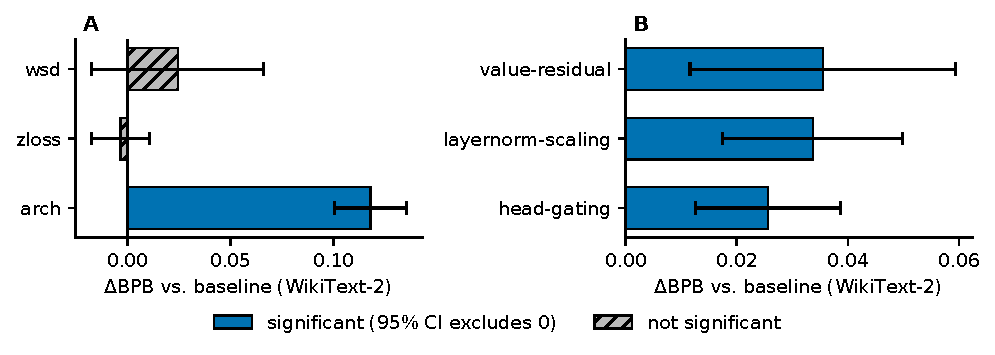
\includegraphics[width=\linewidth]{figures/fig_deconfound.pdf}
\caption{De-confounding the IMU-1 bundle on WikiText-2 BPB improvement over
the faithful AdamW baseline (positive $=$ better). Panel A: Phase-1 axes --
wsd (schedule), zloss (regularizer), arch (the three-flag architecture
bundle). Panel B: Phase-2 sub-drill of the arch bundle into value-residual,
layernorm-scaling, and head-gating, scored against the reused Phase-1
baseline checkpoints. Every cell trains $2000$ steps $\times$ $65{,}536$
tokens $= 131{,}072{,}000$ tokens; $n{=}3$ seeds per arm; error bars are
95\% CIs; hatched grey bars are not significant. Iso-FLOP holds within the
5\% gate for all arms (largest deviation $+0.077\%$ parameters, FLOP ratio
1.00043); all numbers are \texttt{text-lm-v2}-stamped. Sources:
\texttt{verdict.json} of experiments
\texttt{2026-06-18\_qwen3-0.6b\_imu1-deconfound-p1} and
\texttt{2026-06-21\_qwen3-0.6b\_arch-subdrill-p2}, plotted by
\texttt{fig\_deconfound.py}.}
\label{fig:deconfound}
\end{figure}

\subsection{De-confound Phase 2: splitting the architecture bundle}\label{sec:pretrain-p2}

Phase 2 drills into the winning arch axis, ablating its three flags
individually -- value-residual (vr), layernorm-scaling (ln), and head-gating
(hg) -- at the same $131{,}072{,}000$ tokens per cell and 3 seeds per arm
(9 new cells). Rather than re-training a baseline, Phase 2 reuses the
Phase-1 baseline checkpoints (identical optimizer, schedule, budget, seeds,
and data) and re-scores them in-cohort, so every comparison shares one
control. Iso-FLOP again holds by a wide margin: value-residual adds 84
parameters, layernorm-scaling adds none, and head-gating adds $458{,}752$
($+0.077\%$, FLOP ratio 1.00043).

Each flag is individually significant on both corpora
(Figure~\ref{fig:deconfound}, panel B; Table~\ref{tab:attrib}): on WikiText-2,
value-residual $+0.0355$ BPB (95\% CI $[+0.0116, +0.0594]$),
layernorm-scaling $+0.0337$ (95\% CI $[+0.0175, +0.0498]$), and head-gating
$+0.0256$ (95\% CI $[+0.0125, +0.0386]$), all at 3 seeds, paired; the code
corpus shows the same pattern at larger magnitudes (Table~\ref{tab:attrib}).
The three single-flag WikiText-2 effects are near-additive: their sum,
$\approx$0.0947 BPB, approaches the bundled arch effect of $+0.1179$ BPB from
Phase 1, leaving only a small residual for interactions and seed noise. The
Phase-2 verdict is again ``attributed,'' with drivers $=$ [vr, ln, hg].

\subsection{What the headline actually was}\label{sec:pretrain-summary}

The attribution chain replaces one unexplained $-17.9\%$ ($n{=}1$, in-loop)
headline with four small, separately measured causes: an optimizer
optimization-speed effect ($+0.47$ BPB at a 42M-token budget, scoped to early
training) and three individually significant architecture effects
(value-residual, layernorm-scaling, head-gating; together $\approx$0.09 of
the $+0.12$ BPB bundled arch gain at 131M tokens) -- while the schedule and
z-loss axes, plausible-sounding members of the same bundle, contributed
nothing measurable at these budgets. None of these attributed effects is a
scale claim; all are 3-seed, iso-FLOP, \texttt{text-lm-v2}-stamped
comparisons at 42M--131M-token proxy budgets on a 596M-parameter model.
